\section{Theoretische Grundlagen}

\subsection{Polygone}
\subsubsection{Definition}

Ein geschlossener  Streckenzug, also eine Folge von Strecken, welche jeweils einen Endpunkt mit ihrem Vorgänger bzw. Nachfolger gemeinsam haben bilden ein \textbf{Polygon}.

\begin{wrapfigure}{hr}{0.25\textwidth}
  \centering
  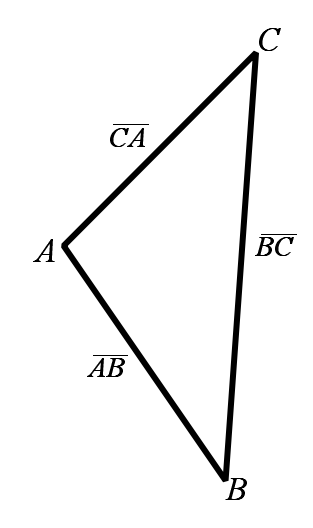
\includegraphics[width=0.2\textwidth]{bilder/dreieck_abc.png}
  \caption[Ein Dreieck als Beispiel für ein Polygon]{\centering Dreick mit Ecken $A, B, C$ als Beispiel für ein Polygon}
  \label{fig:triangle}
\end{wrapfigure}

Dabei ist es wichtig, dass die Anzahl von Strecken endlich ist. "Das Polygon, [zu Deutsch Vieleck], ist also eine durch eine Folge von Strecken begrenzte ebene Fläche." \cite{polydef}
Das einfachste Beispiel hierfür ist ein Dreicke. Es besitzt die Eckpunkte $A$, $B$ und $C$ und wir daher vom Streckenzug aus den Strecken $\overline{AB}$, $\overline{BC}$, $\overline{CA}$ begrenzt (s. Abbildung \ref{fig:triangle}).
Mit genau diesem Prinzip lassen sich beliebig komplexe Polygone erzeugen und beschreiben. Die Strecken werden auch als \textbf{Seiten} und die Endpunkte dieser Strecken 
als \textbf{Ecken} bezeichnet. 
Es sei angemerkt, dass Kreise, obwohl sie ebenfalls ebene Flächen sind, keine Polygone sind. Das folgt daraus, dass Kreise weder Ecken noch eine Begrenzung aus Strecken besitzen.

\subsubsection{Klassifikation von Polygonen}

Es ist denkbar, dass sich die Seiten des Polygons schneiden oder berühren. Man bezeichnet dieses Polygon als überschlagen.\cite{polydef}
Des weiteren kann man Polygone in regulär und nicht regulär unterteilen.
Ein Polygon mit den $n$ Seiten $a,b,c, \ldots$  und den Innenwinkeln $\alpha ,\beta ,\gamma ,\ldots$ heißt regulär, wenn

\begin{center}
  $a=b=c=\dots$ und  $\alpha =\beta =\gamma =\dotsb$
\end{center}
gilt. In einem regelmäßigen Polygon sind demnach alle Seiten zueinander kongruent und alle Winkel gleich groß. \cite{regpoly}

Eine weitere Unterteilungsmöglichkeit lautet wie folgt.
Ein Polygon heißt \textbf{konvex}, wenn für alle Innenwinkel $\alpha _i~(i \in \mathbb{N})$ gilt:
  $\alpha _i < 180^\circ$ 
Anderenfalls heißt es \textbf{konkav}. \cite{convex}

\begin{figure}[t]
  \centering
  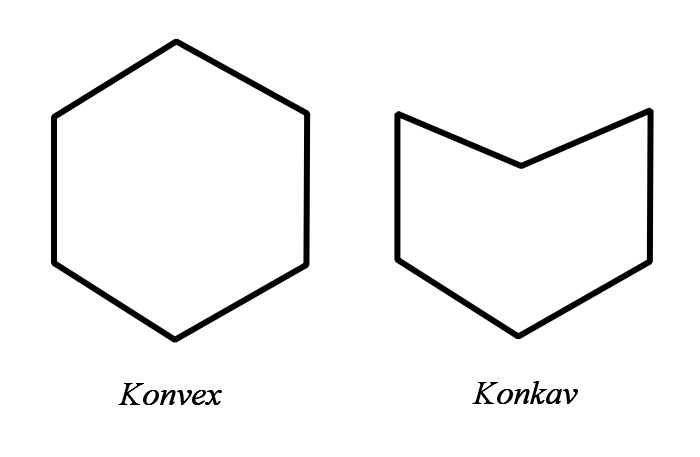
\includegraphics[width=0.5\textwidth]{bilder/konvex_konkav.png}
  \caption[Zwei Secksecke als Beispiel für konvexe bzw. konkave Polygone]{Zwei Secksecke: links konvex, rechts konkav}
  \label{fig:konvexkonkav}
\end{figure}
\pagebreak 
\subsubsection{Diagonalen}

Außer des Streckenzuges, welcher die äußere Grenze des Polygons bildet, kann man im Polygon selbst auch weitere Strecken definieren, 
welche dann als \textbf{Diagonalen} bezeichnet werden. Mittels dieser Diagonalen ist es möglich, jedes Polygon in Dreiecke zu zerlegen. 
Das wird in den nächsten Kapiteln noch näher erläutert, da dieser Sachverhalt die Grundlage für sämtliche Zerlegungsalgorithmen darstellt. 

\subsubsection{Ear und Ear Tips}

Für den in Kapitel 3.3 beschreibenen \ac{eca} ist es der Begriff des \textbf{Ear} (Ohr) relevant. 
Ein Dreieck, welches aus drei aufeinanderfolgenden Ecken $v_{i_0}, v_{i_1}, v_{i_2}$ des Polygons gebildet wird, ohne dass andere Ecken innerhalb 
dieses Dreiecks liegen oder dass der äußere Streckenzug des Polygons durch die Seiten des Dreiecks geschnitten wird, nennt man Ear. Dabei soll die 
Strecke $\left\{v_{i_0}, v_{i_2}\right\}$ eine Diagonale des Polygons. Die Ecke $v_{i_1}$ heißt dann \textbf{Ear Tip}.\cite{meister}

\begin{figure}[h]
  \centering
  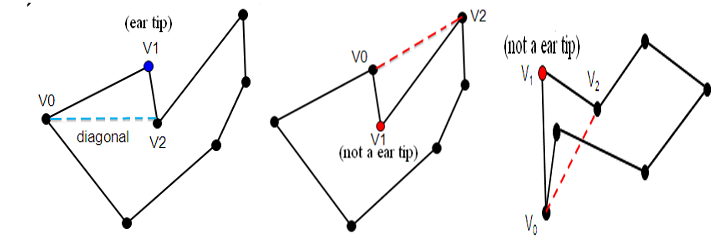
\includegraphics[width=1\textwidth]{bilder/eartips.PNG}
  \caption[Beispiele für Ear und Ear Tips in Polygonen]{\centering Links ist  $\triangle v_{i_0}, v_{i_1}, v_{i_2}$ Ear und $v_{i_1}$ Ear Tip. In der Mitte und rechts 
  ist $\triangle v_{i_0}, v_{i_1}, v_{i_2}$ kein Ear, da $\left\{v_{i_0}, v_{i_2}\right\}$ keine Diagonale ist. \cite{newAlg}}
  \label{fig:ear_eartip}
\end{figure}

\subsubsection{Sätze über Polygone}

Für Polygone gibt es einige Erkenntnisse, welche für die allgemeine Strukturanalyse von eben diesen oder auch für die Triangulation mittels 
\ac{eca} von Bedeutung sind. \break

\begin{flushleft}
  { \textbf{Satz 1 (Jordan'scher Kurvensatz):}

In der euklidischen Ebene $\mathbb{R}^2$ zerlegt jede geschlossene Jordan-Kurve $C \subset \mathbb{R}^2 $ deren Komplement $\mathbb{R}^2 \setminus C$ 
in zwei disjunkte Gebiete, deren gemeinsamer Rand die Jordankurve $C$ ist und deren Vereinigung zusammen mit die ganze Ebene $\mathbb{R}^2$ ausmacht.
\linebreak Genau eines der beiden Gebiete, das sogenannte \textbf{Innengebiet}, ist eine beschränkte Teilmenge von $\mathbb{R}^2$.
\linebreak Das andere dieser beiden Gebiete ist das sogenannte \textbf{Außengebiet} und unbeschränkt. \cite{jordan}
}
\end{flushleft}

\begin{flushleft}
{ \textbf{Satz 2 (Dreieckszerlegung:)}
  
  Jedes Polygon $P$ mit $n$ Ecken kann mittels hinzunahme von null oder mehr Diagonalen vollständig in Dreiecke zerlegt werden. \cite{newAlg}}
\end{flushleft}

\begin{flushleft}
  { \textbf{Satz 3 (Anzahl der Diagonalen:)}
  
  Jede Triangulation eines Polygons $P$ mit $n$ Ecken besteht nutzt $(n-3)$ Diagonalen und besteht aus $(n-2)$ Dreiecken. \cite{newAlg}
}
\end{flushleft}

\begin{flushleft}
  \textbf{Satz 4 (Two Ears Theorem:)}
  
  Jedes Polygon $P$ mit $n \geq 4$ Ecken besitzt mindestens zwei nicht überlappende Ears. \cite{twoears}
\end{flushleft}

\subsubsection{Polytope}
Zuletzt sei an dieser Stelle angemerkt, dass ein Polygon die zweidimensionale Ausprägung des topologischen Begriffs des \textbf{Polytops} ist.
Betrachtet man die räumlichen Dimensionen null bis vier in aufsteigender Reihenfolge so sind ein Punkt, eine Strecke, ein Quadrat, ein Würfel und ein Tesserakt.
Dies ist in der nachstehenden Abbildung zu sehen.

\begin{figure}[h]
  \centering
  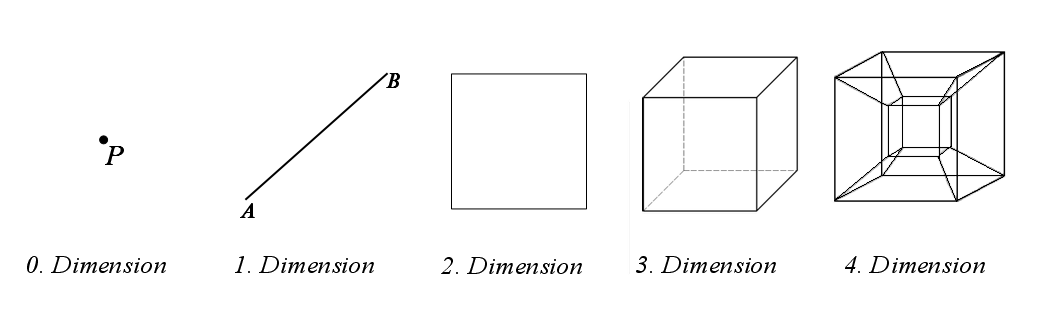
\includegraphics[width=0.9\textwidth]{bilder/Polytope_Dim0_4.png}
  \caption[Beispiele für Polytope der Dimensionen 0 bis 4]{Beispiele für Polytope der Dimensionen 0 bis 4}
  \label{fig:polytope}
\end{figure}

\subsection{Simplexe und Triangulation}

Wie bereits angesprochen kann man durch hinzufügen von Diagonalen in einem Polygon, dieses in Dreiecke oder allgemeiner in Unterpolygone 
zerlegen. Diese Eigenschaft macht sich die \textbf{Triangulation} zu nutze. Allgemein beschreibt der Begriff Triangulation die Zerlegung eines 
topologischen Raumes in \textbf{Simplexe}.\cite{polytri3} Der topologische Raum ist in diesem Fall das Polygon, welches durch einen Streckenzug gebildet wird.

Als Simplex bezeichnet man das einfachste Polygon einer Dimension.\cite{simplex} Für die nullte Dimension ist das trivialer Weise der Punkt. Da keine räumliche Ausdehnung 
möglich ist, ist der begrenzende Streckenzug hier nur der Punkt selbst.
In der ersten Dimension, in welcher Objekte eine Länge aber keine Breite besitzen, ist der Streckenzug eine einzelne Strecke. Diese ist somit auch das Simplex dieser Dimension.
Für die zweite Dimension ist nun das Dreieck das Simplex. Es ist die Fläche, welche aus den wenigsten Punkten, verbunden duch Strecken, erzeugt werden kann und daher das einfachste Polygon dieser 
Dimension. 

Wie bereits beschrieben, kann jedes komplexere Polygon so durch Diagonalen zerlegt werden, dass es volständig von Dreiecken repräsentiert wird. Das ist besonders günstig für 
eine Bearbeitung durch Computer, da ein Dreieck immer eindeutig durch seine drei Eckpunkte beschrieben wird. Diese Form ist daher speichereffizienter als beispielsweise ein allgemeines Viereck, 
für welches nicht nur die Ecken, sondern auch die Kanten gespeichert werden müssten, da mehr als eine Möglichkeit existiert diese vier Punkte zu einem Streckenzug zu verbinden.

Da in der Praxis nicht nur zweidimensionale sondern auch dreidimensionale Objekte eine Rolle spielen, stellt sich die folgende Frage. Kann man diese 3D-Objekte nicht auch in ebenfalls dreidimensionale 
Simplexe zerlegen? 

\begin{wrapfigure}{l}{0.25\textwidth}
  \centering
  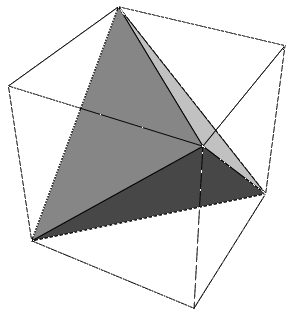
\includegraphics[width=0.2\textwidth]{bilder/cube.png}
  \caption[Zerlegung eines Würfels in vier Tetraeder]{\centering Zerlegung eines Würfels in vier Tetraeder \cite{cubecut}}
  \label{fig:cubecut}
\end{wrapfigure}

Die Antwort ist ja, jedoch ist das nicht sonderlich nützlich. Natürlich existiert in der dritten Dimension auch ein Simplex. Dieses ist der Tetraeder. Man kann auch jedes Polytop 
dieser Dimension in Tetraeder zerlegen, nur benötigt man diese Zerlegung nicht. 
Wöllte man das Innere eines Objektes durch die Zerlegung ebenfalls erhalten, beispielsweise einen Vollwürfel aus Holz in der 
Realität zersägen, dann wäre eine Tetraederzerlegung notwendig. Ein Beispiel für diese Art der Zerlegung ist in Abbildung \ref{fig:cubecut} zu sehen. 
Da man in der digitalen Welt keine echten ausgefüllten Volumina betrachtet sondern nur die Oberfläche darstellt, ist dieses verfahren für die 
Computergrafik uninteressanrt. Man kann die räumlich orientierte Oberfläche eines Würfels topologisch isomorph zu einem Würfelgitter aus quadratischen Flächen beschrieben. Diese Gesamtfläche lässt sich dann 
wiederum in Dreiecke zerlegen. Somit lässt sich auch die Oberfläche dreidimensionaler Objekte durch eine Triangulierung beschreiben. Das ist besonders gut geeigent für Computer, da man nur einen einzigen 
Algorithmus zur Bearbeitung von Flächen und Körpern benötigt, wenn man diese in Dreiecke zerlegen möchte.

\begin{figure}[h]
  \centering
  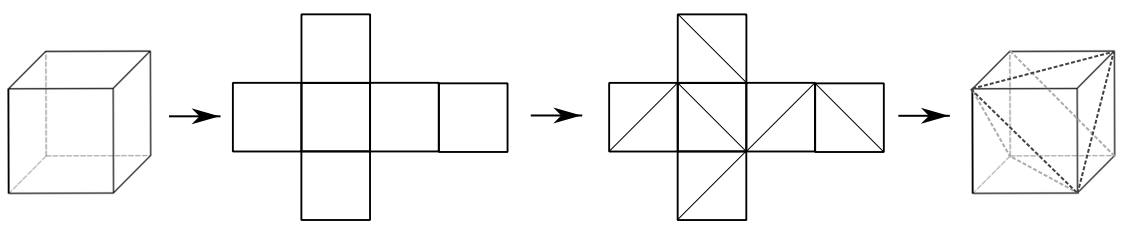
\includegraphics[width=0.9\textwidth]{bilder/3DZerlegung.png}
  \caption[Zerlegung der Oberfläche eines Würfels in Dreiecke mittels Würfelgitter]{\centering Zerlegung der Oberfläche eines Würfels in Dreiecke mittels Würfelgitter}
  \label{fig:cubenet}
\end{figure}

\subsection{Slivers}

Bei Triangulationsalgorithmen wie dem \ac{eca} liegt der Fokus zunächst nicht in der Qualität der Zerlegung. Natürlich gibt es verbesserte Versionen wie beispielsweise in Kapitel 3.1 beschreiben wird.
In jedem Fall sind sogenannte \textbf{Slivers} jedoch ein negativer Einflussfkator, wenn es um qualitative Gesichtspunkte geht. Dreiecke haben in der Computergrfaik die Eigenschaft, dass wenn man eine Scanline 
durch das Dreieck legt, dann schneidet diese ein Dreieck zweimal die Kanten des Dreieck. Diese zwei Schnittpunkte, werden von zwei unterschiedlichen Pixeln auf dem Bildschirm repräsentiert. Somit lässt sich definieren, 
wo eine Fläche beginnt und wo sie endet und dies auf dem Bildschirm darstellen. Bei Slivers ist das nicht der Fall. Ihre Innenfläche ist so schmal,
dass die beiden Schnittpunkte der Scanline mit den Kanten des Dreiecks auf den selben Pixel fallen. \cite{sliverdef} Das führt in letzter Instanz zu Grafikfehlern. 

\begin{wrapfigure}{r}{0.54\textwidth}
  \centering
  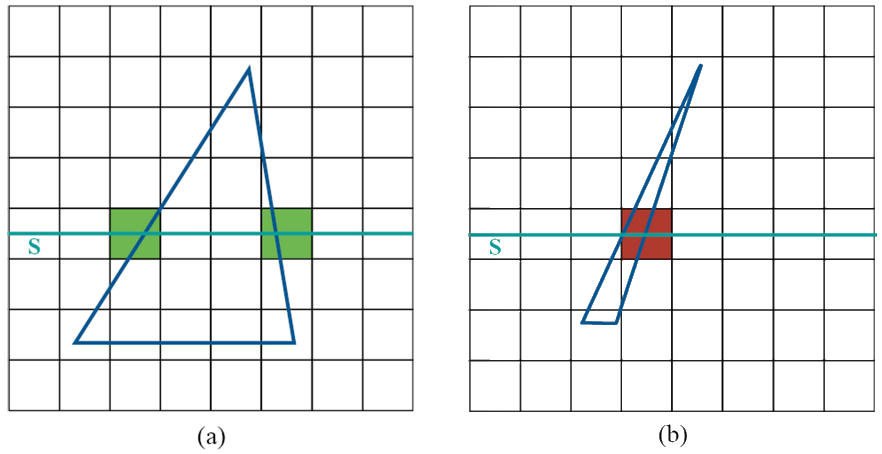
\includegraphics[width=0.49\textwidth]{bilder/sliverScanline.png}
  \caption[Unterschied Sliver und normales Dreieck]{\centering (a) Scanline mit zwei seperaten Schnittpunktpixeln (b) Sliver mit nur einem Pixel für beide Schnittpunkte}
  \label{fig:sliver}
\end{wrapfigure}

Der Begriff Sliver beschränkt sich nicht nur auf Dreiecke. Auch andere Simplexe wie Tetraeder können Simplexe sein. Dass sind diese so flach, dass auch hier Darstellungsfehler entstehen.
Zusätzlich dazu gibt es noch den verwandten Begriff der \textbf{Neadle}, der in Bezug auf Tetraeder, einen sehr schmalen aber auch sehr spitzen solchen bezeichnet.\cite{sliver} \linebreak

\subsection{Der Traditionelle Ear-Clipping-Algorithmus}

Der, in dieser Arbeit, zentrale Punkt, ist der \ac{eca}. Dieser wurde von Meister in seiner Abhandlung \emph{Polygons have ears} \cite{meister} in seiner ursprünglichen Form beschrieben.
Der Algorithmus bestimmt Dreiecke, welche die Eigenschaft eines Ears erfüllen, fügt die dafür nötige Diagonale in eine Liste ein und löscht den Punkt, welcher ein Ear Tip ist aus der Liste aller noch nicht 
bearbeiten Punkte. Dies wird solange wiederholt, bis das Restpolygon nurnoch aus drei Punkten besteht. Zuletzt wird die Lister der Diagonalen ausgegeben, da diese die Triangulation des Polygons erzeugt.
Der Algoritmus ist im Folgenden in Pseudocode dargestellt.

\begin{flushleft}
  { \textbf{Algorithmus 1: Traditionelles Ear-Clipping} \cite{improvedeca}
        \begin{tabbing}
          \=$~~~~~~$\= \textbf{Eingabe:} $~~~$\= Polyg\=on $P$ mit $n$ Ecken in einer Liste $L$\\
          \> \> \textbf{Ausgabe:} \> Liste $D$ mit $n-3$ Diagonalen, die eine Triangulierung bilden.\\
          \> \> \textbf{Schritt 1:} \>Sei $D := \emptyset$ Liste der Diagonalen.\\
          \> \> \textbf{Schritt 2:} \>\textbf{while} $|L| > 3$ \textbf{do}\\
          \> \>                     \> \> (a) Finde ein Ear $v_{i-1}, v_i, v_{i+1}$\\
          \> \>                     \> \> (b) $D := D \cup \left\{v_{i-1} v_{i+1}\right\}$\\
          \> \>                     \> \> (c) $L := L\setminus v_i$\\
          \> \> \> \textbf{endwhile}\\
          \> \> \textbf{Schritt 3:} \> Ausgabe von $D$ als triangulierende Diagonalen.
        \end{tabbing}
}
\end{flushleft}

Dieser Algoritmus hat einen Zeitaufwand von $O(n^3)$ mit einem Aufwand von $O(n^2)$ für das Ermitteln des Ear-Status eines Dreiecks. 
In dieser Formulierung wird nicht auf die Klassifikation eines Ears im speziellen eingegangen. Hierfür beginnt man klassisch 
beim ersten ersten Punkt in $L$. Man überprüft ob dieser Punkt $v_i$ konvex ist. Ist das der Fall, dann muss die Strecke $\left\{v_{i-1}v_{i+1}\right\}$ die Eigenschaft haben, 
eine Diagonale von $P$ zu sein. Wenn das ebenfalls zutrifft, dann ist das Dreicke $v_{i-1}, v_i, v_{i+1}$ ein Ear. 
Man kann die Klassifikation so darstellen:

\begin{flushleft}
  { \textbf{Algorithmus 2: Ear Klassifikation}
        \begin{tabbing}
          \=$~~~~~~$ \= \textbf{Eingabe:} $~~~$\=  Ecken \=${v_i, v_{i-1}, v_{i+1}} \in L$  $~~~~~~~~$\= \\
          \> \> \textbf{Ausgabe:} \> $\triangle v_{i-1}, v_i, v_{i+1}$ ist Ear oder nicht.\\
          \> \> \textbf{Schritt 1:} \>\textbf{if} $v_i$ konvex\\
          \> \> \> \>\textbf{if} $\left\{v_{i-1}v_{i+1}\right\}$ ist Diagonale von $P$\\
          \> \> \> \> \>Ausgabe $\triangle v_{i-1}, v_i, v_{i+1}$ ist Ear.\\
          \> \> \> \> \textbf{else} \>Ausgabe $\triangle v_{i-1}, v_i, v_{i+1}$ ist kein Ear.\\
          \> \> \> \> \textbf{endif}\\
          \> \> \> \textbf{else} Ausgabe $\triangle v_{i-1}, v_i, v_{i+1}$ ist kein Ear.\\
          \> \> \> \textbf{endif}\\
        \end{tabbing}
}
\end{flushleft}
Diese Klassifikation könnte man auch zuerst über alle Punkte $v_i$ in $L$ laufen lassen. Man spricht dann von der Klassifikationsphase. 
Danach kann man in einer zweiten Phase, der Cutting-Phase, Dreicke auswählen, welche die Ear-Eigenschaft erfüllen und sich nicht überschneiden, 
und diese dann Abschneiden. Mit diesen beiden Phasen im Wechsel kann man ebenfalls eine Triangulation erreichen. 
O'Rourke beschreibt in seinem Buch einen Ansatz, der einige Zeitersparnis bei diesem Algorithmus bewirkt.\cite{orourke}
Anstatt nach dem Abtrennen eines Ear Tip Punkts den Status jedes Eckpunktes erneut zu überprüfen, muss man nur den Status von $v_{i-1}$ und $v_{i+1}$ erneut betrachten.
Nur diese beiden Punkte sind nämlich vom Abtrennen von $v_i$ beeinflusst. Somit benötigt man insgesamt nurnoch eine Zeit von $O(n^2)$.\cite{newAlg} 
In jedem Cutting-Schritt kann man dann zusätzlich entscheiden, welche Dreieck als nächstes ausgewählt werden soll. So könnte an nur die Dreiecke auswählen, welche einer bestimmten Heuristik entsprechen.
Beispielsweise könnten so nur Dreiecke gewählt werden, bei denen der kleinste Innenwinkel das Maximum aller aktuell verfügbaren Innenwinkel ist. Auf diese Weise ist es denkbar,
dass man Sliver vermeiden könnte. Andere Ansätze sind exemplarisch im folgenden Abschnitt aufgeführt.